\documentclass[11pt]{article}
\usepackage{amsmath}
\usepackage[margin=0.68in]{geometry}
\usepackage{booktabs,enumitem,fancyhdr,graphicx,tabularx,titlesec}
\usepackage[table]{xcolor}
\usepackage[hidelinks]{hyperref}
\graphicspath{{docs/lessons/assets/}{../assets/}}
\hypersetup{pdftitle={ADK Lesson 040: Reflective and Interrupted Light},
 pdfauthor={Kevin Shanahan},
 pdfsubject={Calibration-bound reflective observations and qualified beam edges},
 pdflang={en-US}}
\pagestyle{fancy}\fancyhf{}
\lhead{\textsc{ADK Lesson 040}}\rhead{Reflective and Interrupted Light}
\cfoot{\thepage}\setlength{\headheight}{14pt}
\setlength{\parindent}{0pt}\setlength{\parskip}{5pt}
\setlist{nosep,leftmargin=1.45em}
\titleformat{\section}{\Large\bfseries}{\thesection}{0.5em}{}
\newcommand{\lessonbox}[1]{\begin{center}\fbox{\parbox{0.92\linewidth}{#1}}\end{center}}

\begin{document}
\begin{center}
 {\Huge\bfseries Reflective and Interrupted Light}\\[4pt]
 {\Large Qualify copied optical samples without inventing hardware facts}\\[8pt]
 \textit{Synthetic E0 experiment; powered fixture and bench acceptance gated}
\end{center}
\begin{tabularx}{\linewidth}{@{}>{\bfseries}l X >{\bfseries}l X@{}}
Lesson & 040 --- component & Time & 90--150 minutes\\
Prerequisites & Lessons 007--009 & Board & host replay; Mega sketch is synthetic\\
Evidence & copied trace and policy snapshots &
Status & E0 host integration active; bench open\\
\end{tabularx}

\lessonbox{\textbf{Scope gate.} This lesson qualifies supplied ADC counts and
digital levels. It publishes no powered adapter, wiring table, pin assignment,
or formal schematic. Family names do not establish an electrical identity.
No lux, reflectance, distance, navigation, collision-avoidance, ambient
rejection, or crosstalk claim follows from these policies.}

\section{Two sources, two narrow policies}
\texttt{ReflectiveObservation\-Policy} accepts a reflective sample;
\texttt{BeamObservation\-Policy} accepts a beam sample. They share provenance
and quality vocabulary, but they
are not a universal optical driver. Each pure policy owns copied state only:
no endpoint, resource claim, emitter, interrupt, timer, callback, heap, or
hidden clock.

\begin{center}
% ADK visual: pencil
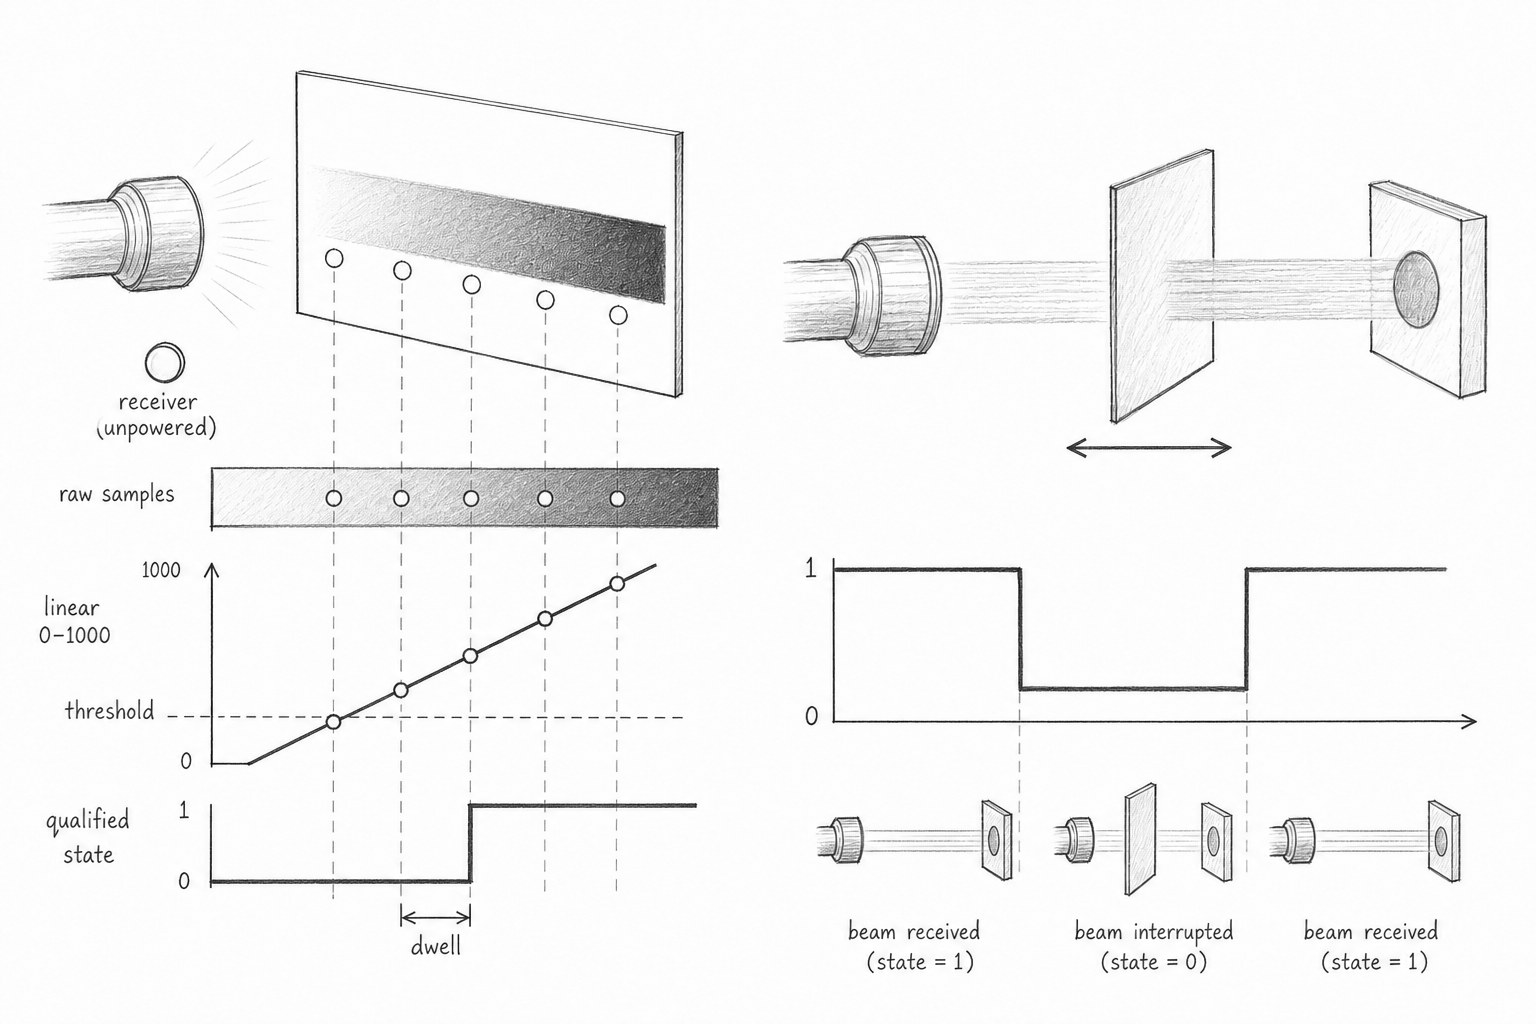
\includegraphics[width=0.96\linewidth]{040-optical-traces-pencil.png}

\small\textit{Alternative text: a graphite worksheet maps five reflective raw
samples through a straight 0--1000 normalization line, then shows a separate
qualified-state step after threshold dwell. Beside it, a hand-moved card
interrupts an abstract beam and produces a high/low trace for one configured
polarity. The drawing is conceptual, unpowered, and not an electrical
schematic.}
\end{center}

The caller supplies \texttt{OpticalProvenance}: source ID, calibration
revision, and observation time. Identity is typed. Equal numeric IDs from a
reflective and interrupted source never mean that the sources are the same.

\section{Normalize reflective evidence}
A valid reflective configuration names a qualified ADC interval, two distinct
references inside it, activation and release thresholds, dwell, and active
polarity. Widened integer arithmetic maps the references onto 0--1000 and
clamps beyond them:
\[
 N=\operatorname{clamp}\left(
 \frac{1000(\mathrm{raw}-\mathrm{darkReference})}
 {\mathrm{lightReference}-\mathrm{darkReference}},0,1000\right).
\]
The implementation handles either reference ordering without unsigned
underflow. The raw count and both references remain in every observation.

Activation and release are separate hysteresis boundaries interpreted relative
to \texttt{darkerIsActive}. A candidate must remain continuously on its side
of the threshold for the configured dwell. The output
\texttt{markerActive} is polarity-independent; later policy never needs to
reconstruct the circuit's direction.

\begin{tabularx}{\linewidth}{@{}l X@{}}
\toprule
Quality & Meaning\\
\midrule
\texttt{Unqualified} & initialized or reset, with no qualified observation\\
\texttt{Valid} & source status, range, calibration, and time are acceptable\\
\texttt{BelowQualifiedRange} / \texttt{AboveQualifiedRange} &
raw evidence is outside the configured interval; no electrical diagnosis\\
\texttt{DegenerateCalibration} & the supplied references cannot define a span\\
\texttt{SourceFault} & the copied source status or level is unusable\\
\texttt{TimingFault} & supplied timestamps violate the deterministic order\\
\bottomrule
\end{tabularx}

\section{Qualify interrupted-light edges}
The beam policy maps one configured digital level to
\texttt{interrupted}. It uses independent interruption and restoration dwell
times. Pulses shorter than a boundary, bounce, and chatter do not become
qualified edges. An edge event lasts for one observation and clears on the
next later update.

The words ``beam'' and ``interrupted'' are semantic labels for copied
evidence. A digital level cannot establish an emitter's wavelength, current,
geometry, range, eye safety, pull-up, or output rail. It also cannot establish
that a retail tracking or avoidance board is electrically equivalent.

\section{Time before interpretation}
Time validation precedes enum, source, range, and threshold processing.
Identical same-time samples are idempotent. Changed same-time evidence,
backward apparent time, or an exact-or-greater unsigned half-range jump
publishes \texttt{TimingFault} without partially applying the changed sample.
Reset clears candidates, edge events, and prior qualification.

\lessonbox{\textbf{Deterministic rule.} A saved configuration, timestamp
sequence, raw samples, and source statuses must reproduce every field exactly.
Sampling between supplied timestamps is unknowable and must not be invented.}

\section{Predict, observe, interpret}
\begin{enumerate}
 \item Replay a slow darkening ramp. Predict that crossing the activation
       threshold alone is insufficient; the complete dwell must also pass.
 \item Observe raw count, normalized value, stable duration, and the one-update
       activation event. Interpret the event only as calibration-bound marker
       evidence.
 \item Reverse the ramp. Predict retention inside the hysteresis band and
       release only after the distinct release threshold and dwell.
 \item Replay one beam pulse just shorter than interrupt dwell and one exactly
       equal to it. Predict suppression, then one interruption event.
 \item Supply changed evidence at the same timestamp. Predict
       \texttt{TimingFault} with no partially updated observation.
 \item Reset and replay the trace. Compare every output field, not only the
       final boolean state.
\end{enumerate}

For this E0 lesson, the copied trace and snapshot table are the non-Serial
observation path. A future powered circuit must add independent raw,
qualified-event, and ready/fault signals. Initialization evidence and
electrical safe-state evidence remain separate checks.

\section{Fault and comparison lab}
Test both reference orderings and active polarities. Exercise each qualified
range edge at minus one, exact, and plus one; each threshold boundary; dwell at
short, exact, and long durations; same-time replay; rollover; half-range; and
reset recovery. Use paired ambient traces and adjacent-source traces only to
compare recorded evidence. Correlation is not proof of ambient compensation or
crosstalk.

An out-of-range ADC result cannot distinguish open, short, floating wire,
surface material, distance, or illumination. A stuck digital level cannot
distinguish a stationary card from a source, receiver, wiring, or adapter
fault. Those diagnoses require an exact powered circuit and measured evidence.

\section{Powered-work gate and open acceptance}
Before any physical adapter, wiring table, formal schematic, or E1 example is
published, one exact specimen must establish markings, pin order, supply,
output rails, polarity, pull-ups, emitter behavior, current, and an
authoritative electrical source. \texttt{Laser Emit} remains excluded and
unpowered.

On a future qualified bench, record unpowered identity and continuity first;
then supply and output ranges, per-path and aggregate current, raw and event
test points, failure behavior, shutdown, reset, and power removal. Stop for
heat, odor, reset, unstable rail, or an unexpected output. Compilation,
deterministic replay, and this PDF are not physical acceptance.

\section{Software evidence and next use}
The deterministic tests cover configuration, ranges, normalization,
hysteresis, dwell, pulse filtering, events, status precedence, time order,
rollover, and replay. Lesson 041 will consume copied qualified evidence while
retaining its source identity, status, age, and disagreement; it will not
requalify these optical samples.

The canonical HTML lesson links the public header, sketch, governing design
record, testing contract, PDF policy, and safety model. This untagged print
edition is its bench companion and makes no PDF/UA or physical accessibility
claim.
\end{document}
